% S&A Latex Template for Assignment Docs
% Reinhold Preiner, 2024
%-------------------------------------------------------------------

\documentclass{article}
\usepackage[utf8]{inputenc}
\usepackage{hyperref}
\usepackage{cite}
\usepackage[english]{babel}
\usepackage{hyperref}
\usepackage{subfig}
\usepackage{graphicx}
\usepackage{float}

\usepackage{geometry}
\geometry{margin=1in}

\hypersetup{
    colorlinks=true,
    linkcolor=blue,
    filecolor=magenta,      
    urlcolor=cyan,
    citecolor = black,
}

\setlength{\parindent}{0pt}
\setlength{\parskip}{0.5em}

\usepackage{comment}

\title{	
	\large Simulation \& Animation - SS 2025\\
	\Huge{Binding of glass Mini golf 2}\\
	\huge{Can you hit it?}
}
\author{\parbox{\textwidth}{\centering
	Florian Winston, 11727495, winston@student.tugraz.at\\%
	Leon Tiefenboeck, 11919874, tiefenboeck@student.tugraz.at\\%
}}
\date{\today}


\begin{document}

\maketitle

\begin{figure}[H]
    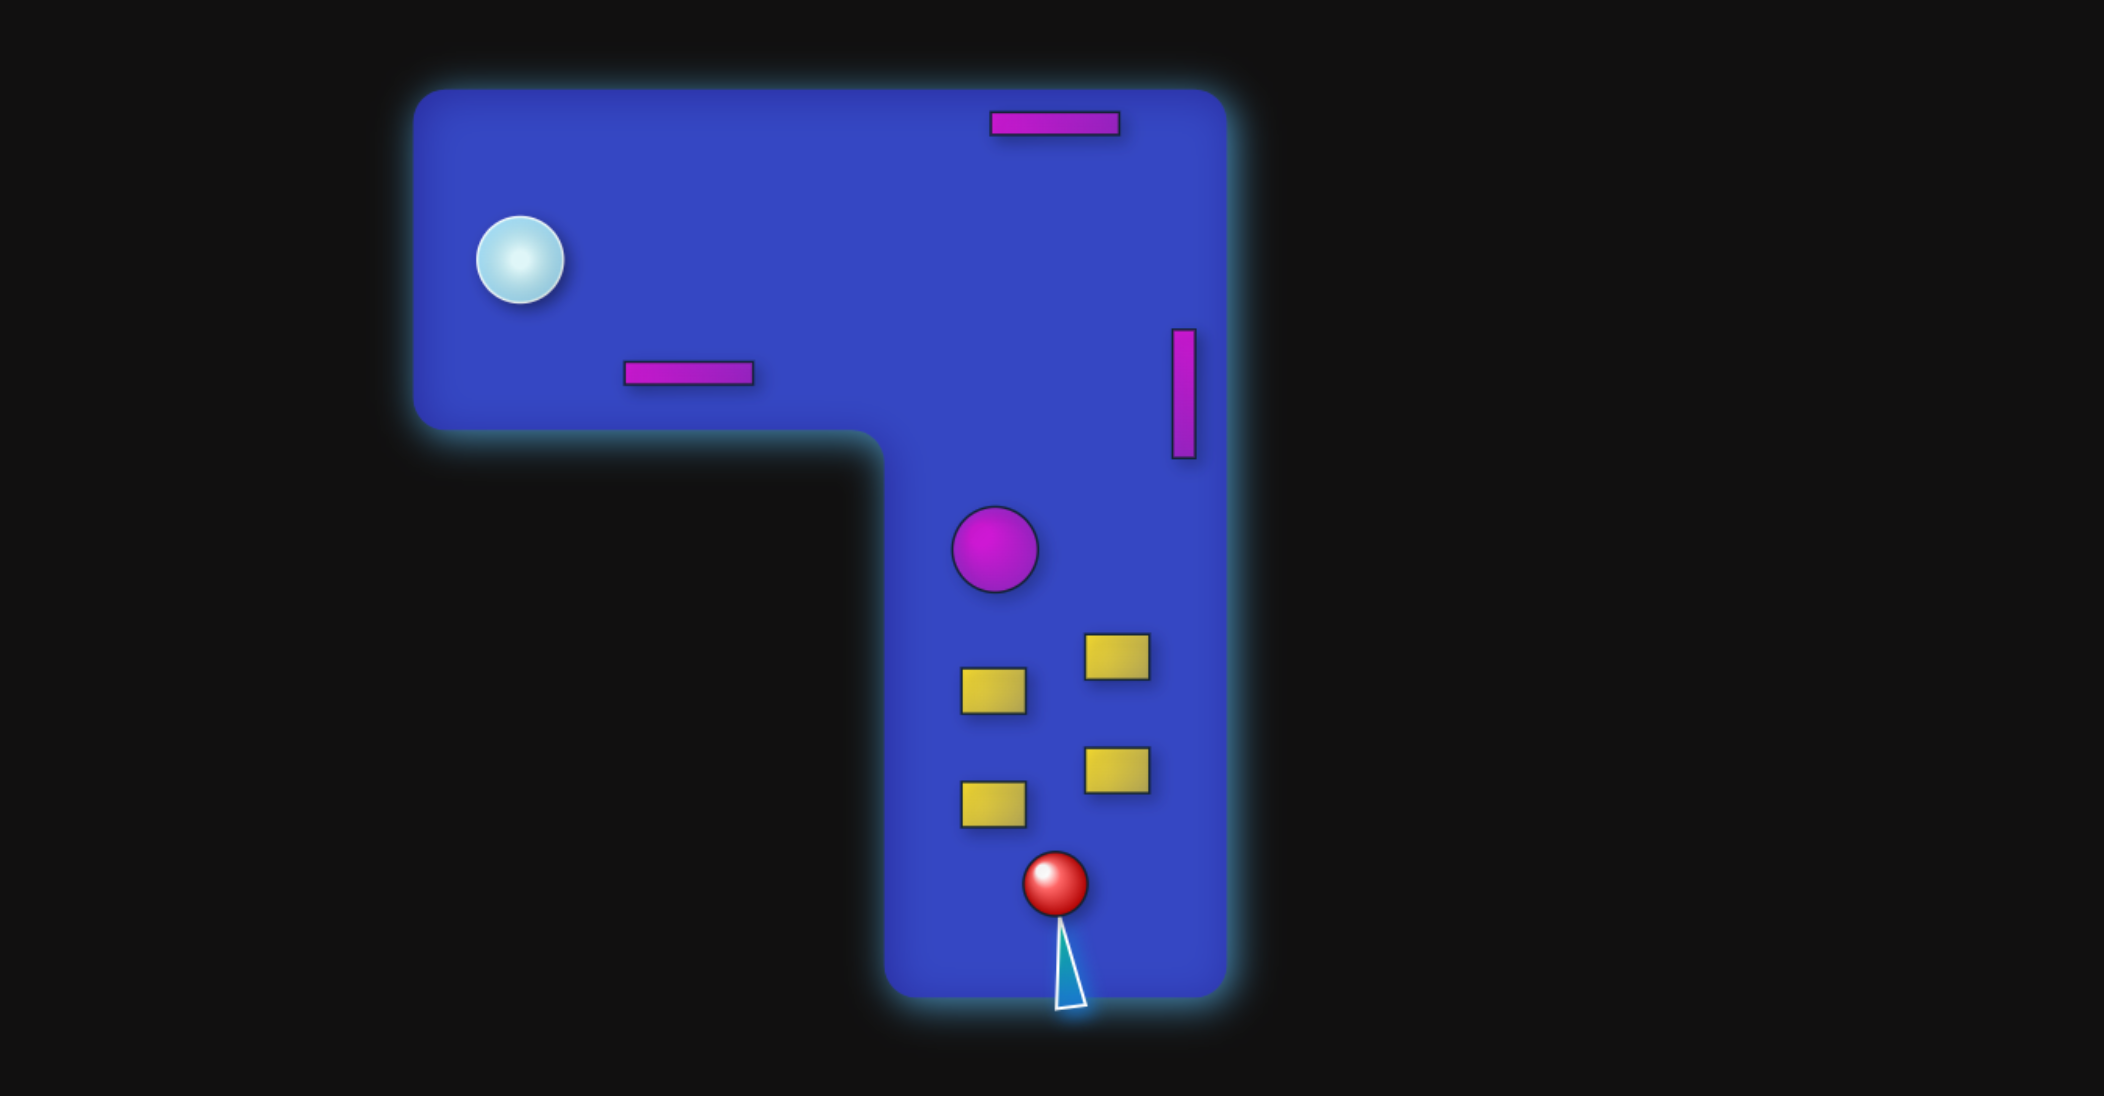
\includegraphics[width=\textwidth]{showcase.png}
    \caption{Screenshot of level 2}
\end{figure}

\section{User Documentation}

\subsection{Gameplay Overview}

Our game consists of three playable levels which feature different techniques: the first contains rigid body collision and path interpolation, the second particle dynamics and the third Voronoi fracture. 
The main concept is the same in all levels, namely putting the small red ball into the white glowing hole. 
In each level this is achieved by using the respective technique.

\subsection{Controls}

The game is started by opening \texttt{main.html} which opens a 
start screen where one can choose between the three levels. 

When starting a level the ball can be seen at the bottom of the screen. This ball can be moved 
by clicking it, dragging somewhere and then releasing the mouse button. 
The ball will move in the opposite direction of where the cursor was dragged and the momentum of the 
ball depends on how far back it was dragged, much like a spring. This is indicated by an arrow that appears below the ball.
Somewhere else in the game area there is a hole, which, to set it apart from the other game objects, 
is very bright and glows a little bit. This is the hole 
the ball should go into. If the player manages that, the level is completed.
On the left side of the screen there is the control panel where level specific techs 
and the overall animation rate and render rate can be adjusted. Here one can also toggle the visualizations 
for different techs. 
Lastly the game can be paused by pressing the \texttt{Escape} key and resumed by pressing it again.

\section{Technical Documentation}

\subsection{General Remarks}
We implemented our game in a very modular way. We have two similar game classes that control the game logic. There are two, since we realized that using different classes would be simpler than making one class work for all techs. These classes include the main loops that 
update the position of objects and render them. We can very easily add other objects from other parts in the 
code to this loop. We can adjust the animation update rate here 
by simply adding a delay to when the next iteration of this loop is called. 
We achieve the frame rate independence here as well, by calculating how long a frame took to produce 
and then adjusting all updates by this delta. 

Next we have an individual class for each of the techs. Here everything should 
also be confined and other parts of the game need only interact with the constructor
and the \texttt{update} and \texttt{render} methods.

Finally, we have a file for each level that interacts with the main game 
class and the different techs. Here we set up
the game objects that are controlled by a tech and their controls (visualization, speed adjustment, etc.).

One thing to note is that we tried to make the game render the same on different displays, so we used 
positions and sizes that are relative to the size of the canvas. This works, however, the speeds and forces and so 
on are still in absolutes so the might differ on different displays.

\subsection{Techs}



\subsubsection{Path Interpolation}

This is shown in level 1. Some of the objects (colored in pink) are moving along a spline path. 
To construct a spline we basically only need the control points, that an object should go through, and an 
object that moves along this spline. Here theoretically we could always just draw a simple circle but 
for our game we wanted that the main ball can bounce off the path interpolated objects, so we used stationary rigid bodies
as the moving objects. More on this later, but these are basically rigid bodies that can only 
exert forces on other objects but do not move themselves, i.e. their entire movement is controlled by the spline.

For our splines we also have the option to change the traversal speed, to loop them or move them back and forth and 
to use easing function to move the objects at non-constant speeds.

For the interpolation we use Catmull-Rom with arc length parametrization. At the start 
we precompute a lookup table that maps the arc length s of the spline to the t values, that we use for the interpolation.
Each time \texttt{update} is called, we calculate the new value based on the current s value, the delta time and the traversal speed, then we make the 
lookup in the arc length table and evaluate the spline at that value. This is done by 
calculating the current segment of the spline, which we then use to index the control points, where we need 4 in each segment
to then use the Catmull-Rom interpolation formula to get a new point.

\subsubsection{Rigid-Body Dynamics}

This tech is also shown in level 1. Here basically all objects (colored in yellow) that are not controlled by a spline (although as mentioned above these do act as stationary rigid bodies) are rigid bodies, except the hole.
The main ball also is a rigid body, where the player can apply some momentum. 

A rigid body is defined by its position, mass, shape and linear as well as angular momentum. 
We can freely set the position and shapes, but the mass is calculated based on the shape and a constant density factor.
With the mass we also calculate the inertia, where we took the formulas from Wikipedia (referenced in the code).

We implemented the rigid bodies as a class, with two subclasses where each represents a different shape, namely circles and rectangles.
The main class takes care of the updating, where we calculate the new position and velocity
based on the current position velocity and all forces acting on the body using Velocity Verlet integration. 

\[
    p_{t+1} = p_{t} + v_{t} \cdot \Delta t + 0.5 \cdot a_{t} \cdot \Delta t^2 
\]
\[
    v_{t+1} = v_{t} + 0.5 \cdot a_{t} \cdot \Delta t
\]

In each update we also apply some linear as well as angular drag by adding a force that points in the opposite direction
of the current velocities and is scaled by a drag factor.
In the subclasses all the shape specific calculations, like rendering and collision detection, are done.
We have three methods for collision detection: one for two rectangles, one for two circles and one for 
a rectangle and a circle. 
Since for the assignment only rectangles are necessary, I will only go into detail about those. 
We test a collision between two rectangles via SAT (Separating Axis Theorem), since our bodies are not axis aligned and 
can be rotated. SAT works by projecting the corners of both rectangles onto axes that are the normals 
of the eight edges of the rectangles. If the projections overlap on all axes, then the rectangles are colliding.
We resolve the collision by first separating the rectangles along the minimum translation vector (MTV) and then 
calculating and applying the resulting linear and angular impulses.
For this we use the formulas from the slides and approximate the contact point by just taking the midpoint of the two centers of the rectangles, which
works well enough for our game.

\subsubsection{Particle Dynamics}
Level 2 showcases particle dynamics. Here there are several repelling bodies in red and attracting bodies in purple. Once the ball is shot, they start affecting it. The force field created by the bodies and trajectory of the ball over the last few seconds can be visualized through the button. One can also change the integration method to choose between the RK4 and Euler methods. Only the ball is effected by the forces, while there is no effect on the other object from each other or from the ball.  \newline

The code for this is located in the ParticleDynamics.js file. There, the particle class with the necessary members is defined. It also holds the defineForces function, which takes all the particles into account, to calculate the effect they have onto the ball. The Rk4 and Euler functions are used for the integration step and apply the results to the ball. The visualize and drawArrow functions are used to draw the particles, the trail and the force field. 
Note: Pushing the visualization button once visualizes the trail, pushing again adds the field. Pushing a third time only visualizes the field and pushing a fourth time turns the visualization off again. 
A vector class is also defined, which will be integrated into the other techs. 

\subsubsection{Voronoi Fracture}
Level 3 showcases the Vornonoi Fracture. The fractured object is an octagon. When the ball gets close to it, the process of fracture starts. The visualization button can be used after the object fractures. It first shows the seed points, then the intersection of the distance field between the mesh and the Voronoi distance field. When hit again, first the seed points and then the field are deactivated. The visualization is only available after the collision, since the slides specified, that the fragmentation calculations should be performed at runtime after impact. The toggle noise button can be pressed before the collision to enable or disable the fracture with noise in the Voronoi fields.

The code for this is located in VoronoiFracture.js. There the "Voronoi" class is defined which holds all the necessary data and methods. On start the image for the object is loaded. Once the ball is close enough to the object and impact occurs, the Voronoi seeds are distributed randomly in a bounding box around the object and Perlin noise with the same bounding box is calculated. Next, the SDF is calculated by iterating over all pixels in the bounding box and finding the distance to the nearest border. Here the noise is added to the location of the pixels. After that the mesh of the object is defined and its SDF calculated. Next, the intersection of both SDFs is created and used to calculate which pixels belong to which fragment. Each pixel gets its color values from the corresponding spot on the image. Finally, the fragments are assigned random velocities, which are scaled with the animation rate. Through this, after impact the object fragments with each part moving seemingly randomly.

\section{References}

We mostly consulted the lecture slides for the techs. We also want to note that AI was 
used for help, especially with the very syntax specific drawing methods of the html canvas.


\end{document}